% !TeX spellcheck = it_IT
\documentclass[italian,11pt,a4paper,twoside,openright]{book}
\usepackage[lmargin=142pt,rmargin=95pt,tmargin=127pt,bmargin=123pt]{geometry}
\usepackage[utf8]{inputenc}
\usepackage{graphicx}
\usepackage{siunitx}
\usepackage{babel}
\usepackage{mathtools}
\usepackage{amsmath}
\usepackage{amssymb}
\usepackage{pgf,tikz}
\usepackage{hyperref}
\usepackage{minted}
\usepackage{tabu}
\usepackage{cleveref}
\usepackage{float}
\usepackage{cite}
\usepackage{enumitem}
\usepackage{microtype}
\usepackage{setspace} % for \setstretch
\usepackage[T1]{fontenc}
\usepackage{lmodern} % \scshape
\usepackage{titling} % \thetitle
%\usepackage[nottoc,numbib]{tocbibind} % biblio in index


\setlist[itemize]{noitemsep, topsep=5pt, leftmargin=*}
	
\usetikzlibrary{matrix, positioning, arrows.meta}
\newlength{\myheight}
\setlength{\myheight}{2.5cm}
\tikzset{labels/.style={font=\sffamily\scriptsize},
	circuit/.style={draw,minimum width=2cm,minimum height=\myheight,very thick,inner sep=1mm,outer sep=0pt,cap=round,font=\sffamily\bfseries},
	triangle 45/.tip={Triangle[angle=45:8pt]}
}


\newcommand{\code}[1]{\texttt{#1}} 

% Some definitions.
\def\advisor#1{\gdef\@advisor{#1}}
\def\mastername#1{\gdef\@mastername{#1}}
\def\coadvisorOne#1{\gdef\@coadvisorOne{#1}}
\def\coadvisorOneUniversity#1{\gdef\@coadvisorOneUniversity{#1}}
\def\coadvisorTwo#1{\gdef\@coadvisorTwo{#1}}
\def\committeeInternal#1{\gdef\@committeeInternal{#1}}
\def\committeeInternalOne#1{\gdef\@committeeInternalOne{#1}}
\def\committeeInternalTwo#1{\gdef\@committeeInternalTwo{#1}}
\def\committeeExternal#1{\gdef\@committeeExternal{#1}}
\def\degreeyear#1{\gdef\@degreeyear{#1}}
\def\degreemonth#1{\gdef\@degreemonth{#1}}
\def\degreeterm#1{\gdef\@degreeterm{#1}}
\def\degree#1{\gdef\@degree{#1}}
\def\department#1{\gdef\@department{#1}}
\def\field#1{\gdef\@field{#1}}
\def\university#1{\gdef\@university{#1}}
\def\universitycity#1{\gdef\@universitycity{#1}}
\def\universitystate#1{\gdef\@universitystate{#1}}
\def\programname#1{\gdef\@programname{#1}}
\def\pdOneName#1{\gdef\@pdOneName{#1}}
\def\pdOneSchool#1{\gdef\@pdOneSchool{#1}}
\def\pdOneYear#1{\gdef\@pdOneYear{#1}}
\def\pdTwoName#1{\gdef\@pdTwoName{#1}}
\def\pdTwoSchool#1{\gdef\@pdTwoSchool{#1}}
\def\pdTwoYear#1{\gdef\@pdTwoYear{#1}}
% School name and location
\university{University of Padova}
\universitycity{Padova}
\universitystate{Italy}

% School color found from university's graphic identity site:
% http://www.nyu.edu/employees/resources-and-services/media-and-communications/styleguide.html
\definecolor{SchoolColor}{rgb}{0.71, 0, 0.106} % UNIPD red
\definecolor{chaptergrey}{rgb}{0.61, 0, 0.09} % dialed back a little
\definecolor{midgrey}{rgb}{0.4, 0.4, 0.4}

\hypersetup{
	colorlinks,
	citecolor=SchoolColor,
	filecolor=black,
	linkcolor=black,
	urlcolor=SchoolColor,
	pdftitle={Implementazione di un sintetizzatore musicale su scheda Nexys4 DDR}
}


\renewcommand{\frontmatter}{
	\pagenumbering{roman}
	\maketitle
	\frontispiece
	\clearpage
}

\begin{document}

\author{Enrico Lumetti}
\title{Implementazione di un sintetizzatore musicale su scheda Nexys4 DDR}
%\title{Implementation of a musical synthesizer on the Nexys 4 DDR board}
%\title{Sintesi audio su scheda FPGA Nexys 4 DDR}
%\title{Audio Synthesis on the Nexys 4 DDr FPGA board}
%\title{Implementazione di un sintetizzatore MIDI digitale su scheda FPGA Nexys 4 DDR}
%\title{Implementation of a MIDI synthesizer on the Nexys 4 DDR FPGA board}
\advisor{Daniele Vogrig}
\mastername{Ingegneria dell'Informazione}
\date{15 Luglio 2019}


\thispagestyle{empty}
\begin{center}
	\vbox to0pt{\vbox to\textheight{\vfill \includegraphics[width=11.5cm]{resources/unipd-light} \vfill}\vss}
	%\vspace*{\fill}
	\begin{figure}
		\centering
		\includegraphics[height=2.5cm]{resources/unipd-bn}
	\end{figure}
	
	\setstretch{1.5}
	
	\scshape{\Large{\bfseries{Università degli Studi di Padova}}} \\
	\line(1, 0){400} \\
	\scshape{\large{Dipartimento di ingegneria dell'informazione}} \\
	
	\vspace{5pt}
	\scshape{Corso di laurea in}
	\@mastername
	
	\setstretch{3}
	
	\vspace{40pt}
	\scshape{\LARGE{\bfseries{\textcolor{SchoolColor}{\thetitle}}}} \normalsize \\
	\vspace{25pt}
	\vspace{15pt}
	\scshape{Anno Accademico 2018/19} \\
	\scshape{15 Luglio 2019}
	\setstretch{1.2}
	
	\vfill
	\begin{normalsize}
		\begin{flushleft}
			\textit{Relatore} \hfill \textit{Laureando}\\
			\vspace{1pt}
			Daniele Vogrig \hfill Enrico Lumetti\\
			Università di Padova \\
			\vspace{6pt}
			
		\end{flushleft}
	\end{normalsize}
	
\end{center}
\vspace*{\fill}
\singlespacing
\pagenumbering{gobble} 
\cleardoublepage

\pagenumbering{roman}
\chapter*{Abstract}
Il successo dei sintetizzatori in ambito musicale dagli anni 70 in poi è
è stato determinante per l'industria musicale. Grazie alla loro versatilità
i sintetizzatori permettono di riprodurre svariati suoni, spesso
programmabili dal musicista, e ampliano enormemente le possibilità espressive.
Con l'avvento dell'elettronica digitale quasi tutti i sintetizzatori in
commercio hanno cominciato a fare uso di tecniche di sintesi digitale e
dei microprocessori.
In questa tesi ci si propone di realizzare un semplice sintetizzatore 
digitale polifonico e con sintesi a wavetable, comandabile attraverso
il protocollo MIDI.
Per la realizzazione del sintetizzatore si farà uso di una scheda
Nexys4 DDR, contenente una FPGA Xilinx Artix 7, un dispositivo programmabile
molto diverso da un convenzionale processore e programmato attraverso
il linguaggio di descrizione dell'hardware VHDL.

\tableofcontents
\mainmatter
\pagestyle{plain}
\chapter{Descrizione e funzionamento di un sintetizzatore musicale}
Un sintetizzatore musicale permette la riproduzione di suoni di carattere, intensità e frequenza impostabili dal musicista.
L'utilizzo dei sintetizzatori come strumento, sia in studio che dal vivo, si afferma negli anni settanta grazie all'invenzione del \textit{Minimoog}, meno costoso e voluminoso dei sintetizzari a muro degli anni sessanta.
Il \textit{Minimoog} era un sintetizzatore analogico e monofonico, cioè capace di riprodurre solamente una nota alla volta, al contrario dei moderni sintetizzatori detti \textit{polifonici}.
Al giorno d'oggi i sintetizzatori sono per la maggior parte implementati in maniera digitale, e permettono l'utilizzo di una varietà di tecniche di sintesi (aggiungere)
In questa tesi ci occuperemo di un semplice sintetizzatore polifonico, capace di riprodurre forme d'onda campionate e controllabile attraverso il protocollo MIDI, ampiamente diffuso nell'industria musicale.
Il progetto è stato implementato sulla scheda Nexys 4 DDR della Digilent, dotata di una FPGA (aggiungere), di una porta seriale usata per il testing, e di un uscita mini-jack monofonica.

\section{La catena del segnale del sintetizzatore}
L'input di un sintetizzatore viene dato dal musicista, attraverso uno strumento fisico. Lo strumento invia al sintetizzatore un segnale di controllo che specifica quali note suonare, a che intensità, quali sono i parametri dello strumento ecc. A tale scopo è universalmente impiegato lo standard MIDI, che specifica sia il protocollo di comunicazione che le caratteristiche elettriche della connessione fisica.
Il sintetizzatore si occuperà di riprodurre i suoni desiderati. Due caratteristiche fondamentali del suono riprodotto sono la sua frequenza e il suo timbro. Per variare queste due componenti sono disponibili una varietà di tecniche.
In questo progetto ci si avvale della \textit{Direct Digital Frequency Synthesis} per la generazione di una frequenza determinata, mentre si farà uso di una ROM contenente la forma d'onda campionata per ottenere il timbro desiderato.
La riproduzione di più note contemporanamente si ottiene attraverso una fase di \textit{mixing}, per cui le forme d'onda delle note desiderate vengono sovrapposte.
Alla fine della catena è presente l'uscita audio, che nel caso della Nexys 4 è un (aggiungere) a cui verrà fornito il segnale opportunamente codificato in pulse-width modulation (?).

(aggiungere figura)

(fare sottoparagrafo di titolo delay?)
Il tempo che intercorre tra la sollecitazione dello strumento e l'emissione del suono corrispondente viene chiamato ritardo di propagazione o \textit{delay}.
Il feedback uditivo è essenziale ai fini di una performance musicale, per cui il ritardo introdotto dal sintetizzatore
dovrebbe essere il più basso possibile, con un limite indicativo di \SI{5}{\milli\second}.
Allo stesso tempo, il tempo di ritardo non può essere inferiore al tempo di produzione di un campione (??? va spiegato meglio il funzionamento del sintetizzatore prima di poterne parlare).
^^ spostare in capitolo su generazione del segnale


\chapter{Lo standard MIDI}
\label{chap:midi}

\section{Il protocollo di comunicazione e i messaggi MIDI}
Nel protocollo MIDI\cite{midispec} le informazioni e gli eventi vengono trasmessi sotto forma di \textit{messaggi}.
Ogni messaggio è composto da una sequenza di byte ordinata di cui il primo è detto \textit{status byte} e i successivi
vengono detti \textit{data byte}.
Per riconoscere gli status byte dai data byte si impone che il bit più significativo degli status byte sia sempre 1, quello dei data byte sia 0 e
i rimanenti 7 bit possono rappresentare valori da da 0 a 127.
I primi 4 bit dello status byte identificano il tipo di messaggio MIDI, mentre gli ultimi 4 specificano il canale su cui il messaggio ha effetto,
per un massimo possibile di 16 canali.

\begin{figure}
    \centering
    \def\svgwidth{\columnwidth}
    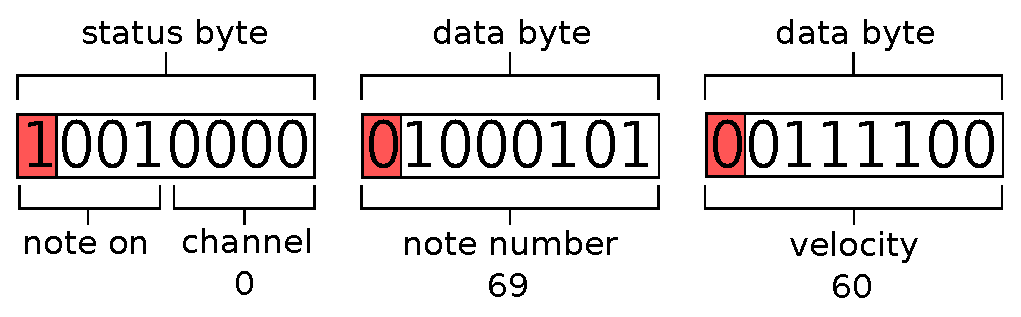
\includegraphics[width=0.7\columnwidth]{TeX_files/midi_message.eps}
    \caption{Struttura di un messaggio MIDI di tipo \textit{note on},
    	     con note number 69 e velocity 60. In rosso è evidenziato
             il bit più significativo.}
\end{figure}

Ai fini del progetto, verranno gestiti solamente i messaggi di \textbf{note on} e \textbf{note off} sul canale '0', mentre
ogni altro tipo di messaggio sarà ignorato.
Ogni messaggio di \textit{note on} viene trasmesso nel momento in cui una certa nota deve essere suonata e contiene due data byte: 
il primo, il \textbf{note number}, identifica la nota da riprodurre, mentre il secondo, detto \textbf{velocity}, fornisce un'informazione
sull'intensità con cui la nota viene suonata. Il suo status byte è del tipo
\textit{1001xxxx} dove \textit{xxxx} sta ad indicare il canale del
messaggio.
Il messaggio note off è analogo e viene trasmesso quando si vuole
interrompere la riproduzione di una certa nota e il suo status byte
ha il formato \textit{1000xxxx}.
Un altro modo di interrompere la nota è quello di mandare
un messaggio \textit{note on} con \textit{velocity} impostata a zero.

\section{Physical Layer}
I messaggi MIDI vengono trasmessi in maniera seriale e vengono ricostruiti da un convertitore seriale/parallelo detto \textit{UART} (Universal Asynchronous Receiver-Transmitter).
La comunicazione MIDI segue il protocollo RS-232 e funziona nel seguente modo:
\begin{itemize}
	\item In assenza di comunicazione, la linea dati viene mantenuta al valore logico alto.
	\item Per iniziare una trasmissione, il trasmettitore porta la linea dati al valore logico basso per la durata $T_{bit}$, e questo valore prende il nome di \textbf{start bit}.
	\item I bit da trasmettere vengono inviati in sequenza, in ordine dal bit meno significativo al più significativo; ad ogni bit corrisponde il valore logico alto o basso sulla linea dati per il periodo $T_{bit}$
	\item Alla fine della tramissione la linea dati viene portata al valore logico alto per un tempo di almeno $T_{bit}$, cioè si invia uno \textbf{stop bit}.
\end{itemize}
Il tempo $T_{bit} = \frac{1}{f_{bit}}$ è definito nello standard MIDI imponendo la frequenza di bit a $f_{bit} = \SI{31250}{\hertz}$, detta anche
\textit{baud rate}.
La sequenza di \textit{start bit}, bit di informazione e \textit{stop bit} compongo il \textbf{data frame} del protocollo MIDI.
Si noti che è necessaria a priori la conoscenza del numero di bit da trasmettere perché la comunicazione abbia successo; nello standard MIDI, ad ogni comunicazione viene inviato un byte e quindi 8 bit.
Il protocollo RS-232 permette anche l'aggiunta di un secondo stop bit e di un \textit{parity bit} per il controllo degli errori, tuttavia questi non sono usati nella comunicazione MIDI.
A differenza del protocollo RS-232 i valori logici alti sono segnalati dallo scorrere di una corrente di $\SI{5}{\milli\ampere}$ invece che dalla presenza di un voltaggio positivo.
Il valore logico basso corrisponde all'assenza di corrente.

\section{Il connettore MIDI}
La prima specifica MIDI prevedeva un connettore DIN a 5 pin, 
con un cavo di lunghezza massima di circa \SI{15}{\meter} usato per trasmettere
la corrente relativa al bit trasmesso.
Sebbene ancora supportato, questo tipo di connettore fisico è stato
soppiantato con l'avvento del protocollo USB e del relativo connettore,
universalmente supportato dai moderni sintetizzatori come mezzo fisico
di trasmissione per i messaggi MIDI.

In questo progetto non si fa utilizzo del connettore MIDI, che dovrebbe essere
interfacciato con un circuito alla scheda; il testing è stato dunque condotto
solamente attraverso l'utilizzo di un computer che comunicasse con la scheda
attraverso la porta USB seriale.

\section{Il MIDI tuning standard}
Ad ogni \textit{note number} del protocollo MIDI viene associata una frequenza determinata dal MIDI tuning standard (MTS).
Date due frequenze $f_2 > f_1$ si dice che distano un'\textit{ottava} se
vale la relazione $f_2 = 2 \cdot f_1$.
Si suddivide ogni ottava in 12 note equidistanziate secondo una progressione geometrica, per cui per ogni nota di frequenza $f$ vale

\[
fs^{12} = 2f 
\]

Da cui si ricava la ragione $s=2^{\frac{1}{12}}$ della progressione geometrica. Moltiplicando una frequenza per $s$ si ottiene la frequenza della nota successiva.
Fissando convenzionalmente la frequenza della nota numero 69 a $ \SI{440}{\hertz}$, si ottiene la corrispondenza tra
il note number $i$ e la frequenza $f$ associata:

\[
f = \SI{440}{\hertz} \cdot s^{i-69}
\]

Dal punto di vista musicale, ogni ottava contiene 12 note, e queste
si ripetono più acute o più gravi passando all'ottava successiva o precedente.
Alla frequenza di \SI{440}{\hertz} si associa convenzionalmente
il "la" da concerto, con cui si accordano gli strumenti di un'orchestra.



\chapter{Dispositivi Hardware della scheda Nexys4 DDR}

L'hardware utilizzato per il progetto consiste in una scheda Nexys4 DDR.

Il nucleo della scheda è costituito da un FPGA Xilinx Artix 7 XC7A100T.
Attorno ad esso sono collegati vari connettori, sensori e pulsanti.

Per la realizzazione del sintetizzatore si farà uso dei seguenti componenti:
\begin{itemize}
    \item \textbf{Bridge USB-UART} Il bridge USB<->UART permette la lettura
          dei messaggi MIDI, inviati dal computer attraverso la porta seriale
    \item \textbf{Mono Audio Output} Un connettore audio monofonico di tipo ??? 
          viene usato per emettere il suono.
\end{itemize}

L'output fornito dal jack audio viene generato attraverso un convertitore analogico/digitale,
costituito da un filtro passa-basso a cui viene fornito in ingresso il segnale
da generare in codifica PWM.

Il filtro passabasso è un filtro di Butterworth del quarto ordine, (Sallen-Key?)
Descrizione di almeno la risposta in frequenza


\section{FPGA}
\subsection{Struttura di un FPGA}
Un Field-programmable Gate Array (FPGA) è un circuito digitale integrato
avente una struttura regolare, e contente:
\begin{itemize}
    \item \textbf{configurable logic blocks}: in breve \textbf{CLB}, blocchi
            logici configurabili che permettono di realizzare funzioni
            logiche arbitrarie
    \item \textbf{configurable routing}: i blocchi logici sono connessi
          attraverso delle connessioni a loro volta configurabili,
          rendendo possibile creare funzioni logiche a un maggior numero
          di ingressi e più complesse
\end{itemize}

Oltre a queste due componenti fondamentali, un FPGA contiente altri
componenti necessari al suo funzionamento e interfacciamento con
circuiti esterni, tra cui:

\begin{itemize}
    \item \textbf{I/O blocks}: blocchi di input e output,
           permettono al FPGA di interfacciarsi con l'esterno
    \item \textbf{Dedicated blocks}: per rendere più efficiente
           l'implementazione di operazioni comuni, esistono vari blocchi
           non configurabili che eseguono funzioni specifiche
    \item \textbf{Memory blocks}: è possibile trovare anche blocchi di
           memoria all'interno di un FPGA
    \item \textbf{Clock Management Tiles e Clock Routing}: circuiteria necessaria per 
           la gestione e propagazione del segnale di clock
\end{itemize}

Il FPGA utilizzato dalla scheda Nexys 4 DDR è uno Xilinx Artix 7 XC7A100T.
Esso contiene 15850 logic slices (ognuno di essi composto da più
configurable logic blocks) e sei clock management tiles (CMT) con
phase-locked loop.
Inoltre, di importanza per il progetto trattato, sono i 240 DSP slices, 
componenti dedicati (semi-configurabili?) che rendono più efficiente
l'implementazione dei sommatori e i 4860 Kbits di Block Ram (BRAM),
che verranno impiegati in fase di sintesi per memorizzare sia la forma
d'onda campionata che le frequency tuning words impiegate nella digital
direct synthesis.

\subsection{Struttura di un CLB}

\section{Programmazione di un FPGA}
La programmazione di un FPGA avviene a livello fisico attraverso
la scrittura di una SRAM che indica come vanno configurati i blocchi
logici e le interconnessioni presenti nell'IC.

A livello di sviluppo si utilizzano linguaggi di descrizione dell'hardware
(HDL) come VHDL e Verilog, che nascondono in gran parte la complessità
dell'FPGA.

Il codice sorgente viene processato da un programma di sintesi che compie
all'incirca le seguenti operazioni:

\begin{itemize}
    \item \textbf{Creazione del netlist}: il codice viene convertito in una
          netlist composta da componenti ad alto livello (come sommatori,
          multiplexer, registri ecc..) che tuttavia è ancora non combacia
          con alla struttura fisica del FPGA
    \item \textbf{Place and Route}: la netlist viene mappata fisicamente sui
          componenti del FPGA
    \item \textbf{Bitstream Generation}: Il risultato del Place and Route viene
          convertito in una serie di bit che vengono poi scritti sulla SRAM
          del FPGA in fase di programmazione
\end{itemize}

In fase di progetto e di sviluppo il design può essere simulato e analizzato
ben prima di passare alla programmazione della scheda.
Un passo particolarmente importante è l'analisi dei tempi di propagazione:
successivamente al place and route è possibile calcolare il tempo di propagazione
del segnale attraverso la logica implementata. Nel caso in cui siano presenti
delle route con un tempo di propagazione troppo lungo, sarà necessario
intervenire a livello del design o addirittura manualmente nel posizionamento
dei blocchi sulla FPGA.

Come verrà descritto più avanti, per questo progetto è stato necessario
modificare l'implementazione del sintetizzatore più volte per garantire il
soddisfacimento dei vincoli temporali, resa difficoltosa dal grande numero
di route necessarie alla polifonia (??? o era per via della memoria dei campioni?)

\DeclarePairedDelimiter\floor{\lfloor}{\rfloor}

\chapter{Sintesi digitale del segnale}

TODO: descrivere brevemente la catena del segnale con un grafico
parlare di teorema di campionamento Nyquist?

\section{Sintesi digital diretta}
La sintesi digitale diretta (Direct Digital Synthesis, Direct Digital Frequency Synthesis, DDS) permette di generare un segnale periodico di frequenza programmabile attraverso un sistema digitale.

In termini formali, si vuole generare un segnale $x(t)$ periodico di periodo ??? di frequenza angolare (?) $2\pi f$, ampiezza tra -1 e 1??? fase iniziale nulla.
..dire come si riconduce un segnale di periodo $T$ generico a un segnale
periodico di periodo $2\pi f$ 
Un sistema di DDS si compone di due blocchi: il \textbf{phase accumulator} (PA), responsabile di generare la fase del segnale a una determinata frequenza, e il \textbf{phase to amplitude convereter} (PAC), che a partire dalla fase ottiene l'ampiezza del segnale.

In un sistema a campioni, il PAC si avvale di una ROM di $2^{\code{M}}$ parole contenente il segnale campionato a \code{b} bit.
Altre tecniche possibili per generare i campioni sono algoritmiche (ad esempio l'algoritmo CORDIC per generare segnali sinusoidali) [TODO]

Il \textit{phase accumulator} è un registro a $\code{N}$ bit il cui valore rappresenta la frazione del periodo $[0, 2\pi]$ in notazione
fixed point. Ad ogni fronte di salita del clock il valore $\code{F}$ del registro viene incrementato di un valore pari alla \textit{frequency tuning word},
sempre di $\code{N}$ bit, che è in relazione biunivoca con la frequenza $f$ desiderata.

Si ricorda che la fase del segnale $x(t)$ al tempo $t$ è definita come
\[
\phi(t) = 2\pi f t
\]

Nella sintesi digitale, la fase al tempo $t$ si ottiene dal registro di fase secondo quando descritto prima:
\[
\phi = \frac{2\pi \code{F}}{2^\code{N}}
\]

Essendo \code{F} a precisione finita, si avrà un errore (TODO: basso) sulla precisione della fase del segnale.

Sommando la frequency tuning word al valore del registro di fase \code{F} si ottiene il nuovo valore \code{F'},
e poiché l'addizione avviene ad ogni periodo di clock $T_{clk}$ i valori della fase del segnale corrispondenti sono
$\phi(t)$ e $\phi(t + T_{clk})$.
Si può quindi ricavare la \code{FTW} imponendo:
\[
\code{FTW} = \code{F'} - \code{F} = 
\floor{\frac{2^\code{N}}{2\pi}\phi(t+T_{clk}) - \frac{2^\code{N}}{2\pi}\phi(t)}
= \floor{2^\code{N} f T_{clk}} = \floor{2^\code{N} \frac{f}{f_{clk}}}
\]

Dove $\floor{\cdot}$ indica la parte intera.

La frequenza effettiva $f_{o}$ del segnale risultante dalla DDS è dunque
\[
f_{o} = \frac{\phi(T_{clk}) - \phi(0)}{2\pi T_{clk}} = \frac{2\pi \code{FTW}}{2^\code{N} 2 \pi T_{clk}} = \frac{\code{FTW}}{2^N} f_{clk}
\]
in generale diversa dalla $f$ desiderata per via dell'errore di troncamento della fase.

... non serve fase iniziale nulla: il registro contenente la ftw permette
di avere fase iniziale non nulla. Parlare della precisione del 
phase accumulator ...
...dire secondo quali condizioni valgono le formule: ad es f minore fclock/2, k < p...

...usare approssimazioni per stimare errore, magari grafico..

Il PAC genera un nuovo campione alla frequenza di campionamento $f_s$.
L'udito umano è capace di percepire frequenza fino a circa $\SI{21}{\kilo\hertz}$, per cui è necessaria una frequenza di campionamento di almeno $\SI{42000}{\hertz}$.

Per ricostruire il segnale in uscita il campione viene processato da un convertitore digitale/analogico, e il segnale a tempo continuo risultante viene infine processato da un filtro passa-basso.

\section{Conversione D/A attraverso PWM}
Per portare il segnale discreto generato attraverso la DDS al dominio analogico si fa uso di una tecnica di modulazione detta \textbf{pulse-width modulation} (PWM).

Per comprendere il funzionamento della PWM si consideri un semplice esempio: si voglia rappresentare un segnale costante $x(t) \equiv x_0$ con $x_0 \in [0, x_{max}]$

Sia quindi $x_{pwm}(t)$ un'onda quadra di ampiezza $x_{max}$, di periodo $T$ e di duty cycle $d=\frac{x0}{x_{max}}$, $d \le 1$:
\[
x_{pwm}(t) = \begin{cases}
	x_{max} & \text{se}\ kT \le t < (k+d)T \\
	0 & \text{se}\ (k+d)T \le t < (k+1)T
\end{cases}
\] 
con $k \in Z$

È noto che questo segnale è sviluppabile in serie di Fourier come: ...

In particolare, il coefficiente $a_0$ è pari alla media del segnale sul periodo, ossia
\[
a_0 = x_{max} \cdot d = x_0
\]

È possibile quindi ricostruire il segnale $x(t)\equiv x_0$ a partire da $x_{pwm}(t)$ passandolo attraverso un filtro passa-basso che rimuova tutte le armoniche diverse da $a_0$.

Nel caso in esame $x(t)$ non sarà costante, ma sarà variabile e rappresenterà la forma d'onda generata dal sistema di sintesi digitale diretta.

Al segnale costante verrà quindi sostituito il segnale a tempo discreto $x(kT), k \in Z$ generato alla frequenza di campionamento $f_s = \frac{1}{T}$ e con valori $0 \leq x(kT) \leq x_{max}$, e in prima approssimazione il segnale $x_{pwm}$ corrispondente sarà
\[
x_{pwm}(t) = \begin{cases}
	x_{max} & \text{se}\ kT \le t < (k + d_k)T \\
	0 & \text{se}\ (k+d_k)T \le t < (k+1)T
\end{cases}
\]
dove $(d_k)_{k \in \mathbb{N}}$ è una sequenza di duty cycle non più costanti ma \textbf{modulati} e dati da
\[
d_k = \frac{x(kT)}{x_{max}}
\]

Tuttavia il segnale PWM è generato digitalmente, quindi supponendo per semplicità $T=1/f_s$ multiplo del periodo di clock $1/f_{clk}$, in un singolo periodo
di campionamento si avrà una successione di $N=\frac{f_{clk}}{f_s}$ impulsi pari a $x_{max}$ (corrispondente ad un valore logico alto) o $0$ (corrispondente a un valore logico basso).
Poiché al fine della modulazione PWM conta solo il valore medio sul periodo, l'ordine degli impulsi non cambia il risultato, anche se cambia la distribuzione delle armoniche nello spettro del segnale.
È quindi possibile rappresentare un numero finito di valori in uscita pari a $N$, e quindi i campioni forniti potranno al massimo avere una risoluzione di $\log_2{N}$ bit.

La modulazione PWM non è lineare e introduce quindi distorsione nel segnale ricostruito.

\newcommand{\code}[1]{\texttt{#1}} 

\newcommand{\blockdiagram}[4]{
	\begin{tikzpicture}[font=\sffamily,>=triangle 45]
         \node [circuit] (item) {};
		
		\matrix[
		matrix of nodes,
		left= of item,
		row sep=\myheight/15,
		nodes={anchor=east}
		] (rightmatr) {
			#3
			\\
		};
		\matrix[
		matrix of nodes,
		right= of item,
		row sep=\myheight/15,
		nodes={anchor=west}
		] (leftmatr) {
			#4
			\\
		};
	
		\foreach \i in {1,...,#1}
			\draw [->] (rightmatr-\i-1) -- (rightmatr-\i-1 -| item.west);
		\foreach \i in {1,...,#2}
			\draw [<-] (leftmatr-\i-1) -- (leftmatr-\i-1 -| item.east);
	\end{tikzpicture}
}


\chapter{Architettura ed implementazione}

L'architettura da sintetizzare su FPGA è stata sviluppata utilizzando il linguaggio VHDL, facendo
ampiamente uso di molte funzionalità della versione VHDL-2008.
Il progetto è stato sintetizzato usando il software Vivado 2018.2 della Xilinx e simulato usando il compilatore/simulatore open-source GHDL.

Dal punto di vista architetturale si può considerare il progetto come composto da due macro-blocchi indipendenti: uno che si occupa di gestire i segnali MIDI dati in input al sintetizzatore, e uno che si occupa di generare il segnale audio in uscita.

Le due componenti sono implementate in logica sincrona e sono collegate da una lookup table che memorizza le note attive. Alla ricezione di un evento MIDI \textit{note on} il bit corrispondente alla nota nella LUT viene portato al valore logico alto, e al seguente istante di campionamento la componente che genera il segnale di output userà questo valore per determinare se suonare o meno la nota.

\section{Componenti fondamentali}
I seguenti blocchi fondamentali corrispondono in VHDL al costrutto di \textit{entity} e veranno analizzati dettagliatamente in seguito:

\begin{itemize}
	\item \hyperref[sec:uart]{uart} Si occupa della ricezione seriale a 31250 baud secondo le specifiche MIDI
	\item \hyperref[sec:mididec]{midi\_decoder}  State machine che codifica i byte ricevuti dal blocco uart in eventi MIDI; gestisce solamente gli eventi note on/off
	mentre scarta tutti gli altri eventi MIDI.
	\item \hyperref[sec:noteslut]{active\_notes\_lut} Tabella di lookup contenente 128 valori booleani che indicano l'attivazione di una nota
	\item \hyperref[sec:phaseaccumulator]{phase\_accumulator} Opera l'accumulazione di fase per la DDS
	\item \hyperref[sec:pwmencoder]{pwm\_encoder} Genere la modulazione PWM corrispondente in uscita
	a partire da un campione fornito in entrata
	\item \hyperref[sec:rom]{rom} Package generico che rappresenta una read-only memory.
	\item \hyperref[sec:synthengine]{synth\_engine} Cuore del sintetizzatore, provvede alla DDS a partire dai valori presenti in active\_notes\_lut, alla phase-to-amplitude conversion attraverso una ROM e al mixing.
	\item synth\_top Entità top del progetto, cioè che contiene tutte le altre entity e le istanzia nel modo corretto, impostando le frequenze di lavoro dei componenti.
\end{itemize}

\section{Blocco UART}
\label{sec:uart}

%\begin{lumos}
%	\luminput{
%		i\_clock \\
%		i\_serial\_input \\
%	}
%	\lumoutput{
%		o\_data\\
%		o\_data\_available
%	}
%\end{lumos}

\begin{center}
	\blockdiagram{2}{2}{
		i\_clock \\ i\_serial\_input
	}{
	    o\_data \\ o\_data\_available
    }
\end{center}

I messaggi MIDI vengono trasmessi in maniera seriale e vengono ricostruiti da un convertitore seriale/parallelo detto \textit{UART}(Universal Asynchronous Receiver-Transmitter).
La comunicazione MIDI segue il protocollo RS-232 e funziona nel seguente modo:
\begin{itemize}
	\item In assenza di comunicazione, la linea dati viene mantenuta al valore logico alto
	\item Per compiere una trasmissione, il trasmettitore porta la linea dati al valore logico basso per la durata $T_{bit}$, e questo valore prende il nome di \textit{start bit}.
	\item I bit da trasmettere vengono inviati in sequenza, in ordine dal bit meno significativo al più significativo; ad ogni bit corrisponde il valore logico alto o basso sulla linea dati per il periodo $T_{bit}$
	\item Alla fine di tramissione la linea dati viene portata al valore logico alto per un tempo di almeno $T_{bit}$, cioè si invia uno \textit{stop bit}.
\end{itemize}
Si noti che è necessaria a priori la conoscenza del numero di bit da trasmettere perché la comunicazione abbia successo; nello standard MIDI, ad ogni comunicazione viene inviato un byte e quindi 8 bit.
Il protocollo RS-232 permette anche l'aggiunta di un secondo stop bit e di un \textit{parity bit} per il controllo degli errori, tuttavia questi non sono usati nella comunicazione MIDI.

Il blocco uart è composto da una finite state machine (fsm) e uno shift register da 9 bit, contenente inizialmente i valori '0' tranne per il bit più significativo che è posto a '1' e funge da sentinella. La lettura della linea dati avviene periodicamente alla frequenza $f = \frac{1}{T_{bit}} = 31250 \si{Hz}$; alla ricezione dello start bit, la fsm entra nello stato di ricezione e si fa avanzare lo shift register leggendo il valore presente sulla linea nel bit più significativo, facendo contemporaneamente slittare gli altri verso destra.
A lettura ultimata, lo shift register sarà avanzato di 8 posizioni e il bit meno significativo dello shift register contiene il bit sentinella; con questo si indica la fine della trasmissione.

\section{MIDI decoder}
\label{sec:mididec}

\begin{center}
	\blockdiagram{3}{2}{
		i\_clock \\
		i\_enable \\
		i\_data \\
	}{
	    o\_message \\
	    o\_message\_available
    }
\end{center}
Il decoder MIDI si occupa di leggere i byte provenienti dal convertitore seriale/parallelo e di convertirli in messaggi MIDI.
In realtà il componente è molto semplificato in quanto interpreta solo i messaggi di note on e note off, mentre scarta ogni altro messaggio MIDI.
Il blocco è implementato attraverso una fsm; quando l'input \code{i\_enable} viene mantenuto alto per un ciclo di clock, la state machine avanza leggendo il byte \code{i\_data} in input.
Quando il messaggio è stato completamente decodificato, l'output \code{o\_message\_available} assume un valore logico alto e il messaggio MIDI è disponibile in uscita al blocco.

\section{Active Notes LUT}
\label{sec:noteslut}

\begin{center}
	\blockdiagram{3}{1}{
		i\_clock \\
		i\_enable \\
		i\_message \\
	}{
		o\_active\_notes\_reg
	}
\end{center}
Quando il segnale \code{i\_enable} è alto per un ciclo di clock, il valore del messaggio midi in input viene letto e il registro \code{o\_active\_notes\_reg} viene modificato in modo che il bit in posizione corrispondente alla nota sia 1 o 0 a seconda che il messaggio sia note on oppure note off.

\section{Accumulatore di Fase}
\label{sec:phaseaccumulator}

\begin{center}
	\blockdiagram{3}{1}{
		i\_clock \\
		i\_rst\_sync \\
		i\_ftw \\
	}{
		o\_phase\_reg
	}
\end{center}
Parlare dei parametri generici
L'accumulatore di fase è un registro che viene incrementato ad ogni ciclo di clock del valore presente in ingresso alla porta \code{i\_ftw}.
È possibile il reset sincrono del registro impostando al valore logico alto il segnale \code{i\_rst\_sync}

\section{PWM Encoder}
\label{sec:pwmencoder}

\begin{center}
	\blockdiagram{2}{1}{
		i\_clock \\
		i\_sample
	}{
		o\_pwm\_signal
	}
\end{center}
L'encoder PWM si occupa di leggere il campione presente alla porta i\_sample alla frequenza $f_s$ di campionamento
Scrivere considerazioni sul range del segnale di uscita, codifica, aritmetica con segno.
Scrivere riguardo ad alta impedenza

\section{Componente ROM}
\label{sec:rom}
Le ftw e la forma d'onda da riprodurre vengono generate attraverso MATLAB e salvate in un file.
Il package generico rom permettere al progetto di avere queste informazioni in fase di sintesi: si specificano i tre parametri \code{word\_bits}, che indica il numero di bit per parola nella memoria, \code{address\_bits}, che indica il numero di bit necessari a indirizzare una parola, e \code{rom\_filename}, che specifica il file testuale da leggere contenente le parole della rom.
Il file deve essere formattato nel seguente modo: ci sono tante righe quanti sono gli indirizzi della memoria, ogni riga è una stringa binaria
di lunghezza fissa e rappresenta la parola memorizzata.
Gli indirizzi partono da 0 (prima riga) e aumentano di un unità ad ogni riga.
È possibile leggere dalla ROM usando la funzione \code{read\_at}, specificando come argomento l'indirizzo desiderato.
\begin{lstlisting}[language=VHDL]
package rom is
  generic (
    word_bits: positive;
    address_bits: positive;
    rom_filename: string
  );
  subtype word_type is std_logic_vector(word_bits-1 downto 0);
  impure function read_at(
     address: in integer range 0 to 2**address_bits-1
  ) return word_type;
end package rom;
\end{lstlisting}

\section{Synth Engine}
\label{sec:synthengine}

\begin{center}
	\blockdiagram{2}{2}{
		i\_clock \\
		i\_active\_notes
	}{
		o\_sample \\
		o\_sample\_ready
	}
\end{center}

Il componente principale del sintetizzatore ha accesso alla LUT contenenti le note attive e genera ad ogni periodo di campionamento
un campione del segnale.

Attraverso il package \hyperref[sec:rom]{rom} vengono rese disponibili a questo componente la forma d'onda campionata e le frequency
tuning word corrispondenti ad ogni possibile nota suonata.
Attraverso il costrutto \code{for .. generate} vengono generati 128 accumulatori di fase indipendenti. Ad ognuno di questi viene accoppiata
una entity che ne esegue il reset quando una nota passa dal valore logico basso a quello alto nella LUT.
\begin{lstlisting}[language=VHDL]
oscillators:
for i in 0 to MAX_MIDI_NOTE_NUMBER generate
    signal ftw: std_logic_vector(phase_bits-1 downto 0);
    signal reset_signal: std_logic := '0';
begin
    ftw <= phase_rom.read_at(i);

    reset_generator: entity work.low_to_high_detector
    port map (
        i_clock => i_clock,
        i_signal => i_active_notes(i),
        o_detected => reset_signal
    );

    accumulator: entity work.phase_accumulator
    generic map (
        clock_frequency => clock_frequency,
        phase_bits => phase_bits
    )
    port map (
        i_clock => i_clock,
        i_rst_sync => reset_signal,
        i_ftw => ftw,
        o_phase_reg => phase_vec(i)
    );
end generate oscillators;
\end{lstlisting}

Il campione viene fornito all'output \code{o\_sample} e viene generato attraverso un processo di mixing.
Il mixing consiste nel seguente processo, ripetuto per ogni valore della LUT delle note attive:
\begin{itemize}
    \item Se la nota è attiva, si carica il valore campionato della forma d'onda ad essa relativa:
          il valore campionato viene ottenuto dalla ROM dei campioni, usando come indice
          i primi ??? bit dell'accumulatore di fase: infatti questo è il
          \textbf{phase to amplitude converter} (PAC)
    \item Il valore del campione viene sommato su un registro inizialmente nullo
\end{itemize} 

Tuttavia, come verrà chiarito in seguito (aggiungere hyperref),
l'implementazione fa uso di una pipeline a due stadi:
il primo stadio della pipeline provvede alla PAC, mentre il secondo stadio
esegue parallelamente il mixing con il valore ottenuto dallo stadio
precedente.

Ogni avanzamento della pipeline viene eseguito in un ciclo di clock,
e in totale sono necessari 129 cicli di clock
(128 per ogni nota, più uno per caricare la pipeline) che vengono eseguiti
appena prima della fine del periodo di campionamento.
Questo avviene all'ultimo ciclo di clock della fase di produzione del
campione, in cui l'output \code{o\_sample\_ready} assume il valore
logico alto per indicare la presenza di un campione.

TODO: commentare sul fatto che c'è ampio margine di tempo, magari calcolare


\chapter{Testing e analisi delle prestazioni}
Il testing del progetto sulla scheda Nexys4 DDR è stato condotto
attraverso la porta seriale della scheda e mediante l'uso di uno
script Python che automatizzasse la riproduzione di un file MIDI 
(si veda \code{scripts/play\_midi\_file.py} (aggiungere citazione al codice).

Per effettuare il testing funzionale delle varie componenti del progetto
si è fatto uso di \textit{testbenches} scritti in VHDL, che fornissero
un input prefissato a un certo componente per verificarne la risposta,
utilizzando sempre GHDL.
In particolare il testbench descritto nel file
 \code{vhdl/mono\_synth\_engine\_tb.vhd} provvede a testare l'intera
architettura riproducendo una singola nota.
L'uscita del blocco \code{pwm\_encoder} viene quindi salvata ad ogni
ciclo di clock su un file txt, che viene in seguito processato
dallo script \code{scripts/plot\_pwm\_output.py} che lo filtra
digitalmente e visualizza il segnale ricostruito.

Data la complessità computazionale di una simulazione, il testbench
di prova dell'intero progetto può impiegare fino a diversi minuti
per generare un output che realmente avrebbe durata nell'ordine della
decina di millisecondi.

\section{Qualità del segnale sintetizzato}


\begin{thebibliography}{9}
\bibitem{sourcecode} 
Codice sorgente del progetto, testbench, latex e scripts.
\href{http://github.com/doppioandante/tesi}{Link Github}.

\bibitem{midispec}
The MIDI association.
\textit{The MIDI 1.0 Specification}

\bibitem{artix7overview}
Xilinx.
\href{https://www.xilinx.com/support/documentation/data_sheets/ds180_7Series_Overview.pdf}{\textit{7 Series FPGAs Data Sheet: Overview}}.

\bibitem{artix7clb}
Xilinx.
\href{https://www.xilinx.com/support/documentation/user_guides/ug474_7Series_CLB.pdf}{\textit{7 Series FPGAs Configurable Logic Block}}

\bibitem{nexys4referencemanual} 
Digilent.
\href{https://www.xilinx.com/support/documentation/university/XUP%20Boards/XUPNexys4DDR/documentation/Nexys4-DDR_rm.pdf}{\textit{Nexys4 DDR FPGA Board Reference Manual}}
% Albert Einstein. 
% \textit{Zur Elektrodynamik bewegter K{\"o}rper}. (German) 
% [\textit{On the electrodynamics of moving bodies}]. 
% Annalen der Physik, 322(10):891–921, 1905.

\bibitem{oppenheim}
Oppenheim, Allan V. and Willsky, Alan S. and Nawab, S. Hamid
\textit{Signals \& Systems (2Nd Ed.)}.
Prenctice-Hall, Inc., 1996.

\bibitem{tlc}
Nevio, Benveuto.
\textit{Principles of Communications Networks and Systems}.
Wiley, 2011.

\bibitem{pwmspectrum}
Song, Sarwate.
\textit{The Frequency Spectrum of Pulse Width Modulated Signals}.
Signal Processing Volume 83, Issue 10, October 2003, Pages 2227-2258.

\bibitem{analogdevicessec4}
Analog Devices.
\textit{A Technical Tutorial on Digital Signal Synthesis}.
Section 4.

\bibitem{exactspurs}
Torosyan, Willson.
\textit{Exact analysis of DDS spurs and SNR due to phase truncation and arbitrary phase-to-amplitude errors}
Proceedings of the 2005 IEEE International Conference.
Frequency Control Symposium and Exposition, 2005. 
\end{thebibliography}


\backmatter
% bibliography, glossary and index would go here.

\end{document}
